\documentclass{beamer}
\usetheme{Madrid}
\usecolortheme{spruce}

\usepackage{pgfplots}

\usepackage{bm}

\usepackage{color}

\usepackage{graphicx}

\graphicspath{{./img/}}

\title{Stochastic Gradient Descent}
\subtitle{STAT 672 Project}
\author{Tom Wallace}
\institute{George Mason University}
\date{Spring 2018}


\begin{document}

\frame{\titlepage}

%%%%%%%%%%%%% Introduction %%%%%%%%%%%%%%

\begin{frame}
	\frametitle{Optimization is fundamental to statistical modeling}
	Suppose that we have a typical supervised classification problem
	\begin{itemize}
		\item \small Non-parametric: no assumptions about distribution of data
		\item Feature vector $\mathbf{X}_i$, label $Y_i$
		\item Want to find best prediction function $f_w^*$ from class $\mathcal{F}$
		\item Optimization: pick weights $\hat{\bm{w}}$ that minimize
			empirical risk according to some convex
			loss function $L(f_w(x), y)$ \\~\\
	\end{itemize}

	Our lack of assumptions takes away some familiar tools for finding $\hat{\mathbf{w}}$
	\begin{itemize}
		\item \small Cannot analytically identify $\hat{\mathbf{w}}$
			(e.g. in OLS $=(X'X)^{-1}X'Y$))
		\item \small Newton-Raphson requires 2nd derivative of $L$,
			which might be a pain (unlike in, for example, GLM)\\~\\
	\end{itemize}

	But we still know that if $L$ is convex, there is a unique global
	minimum, and the gradient at that point must be 0
\end{frame}

\begin{frame}
	\frametitle{Gradient descent is an iterative search procedure}
	\begin{figure}[h]
	\centering
	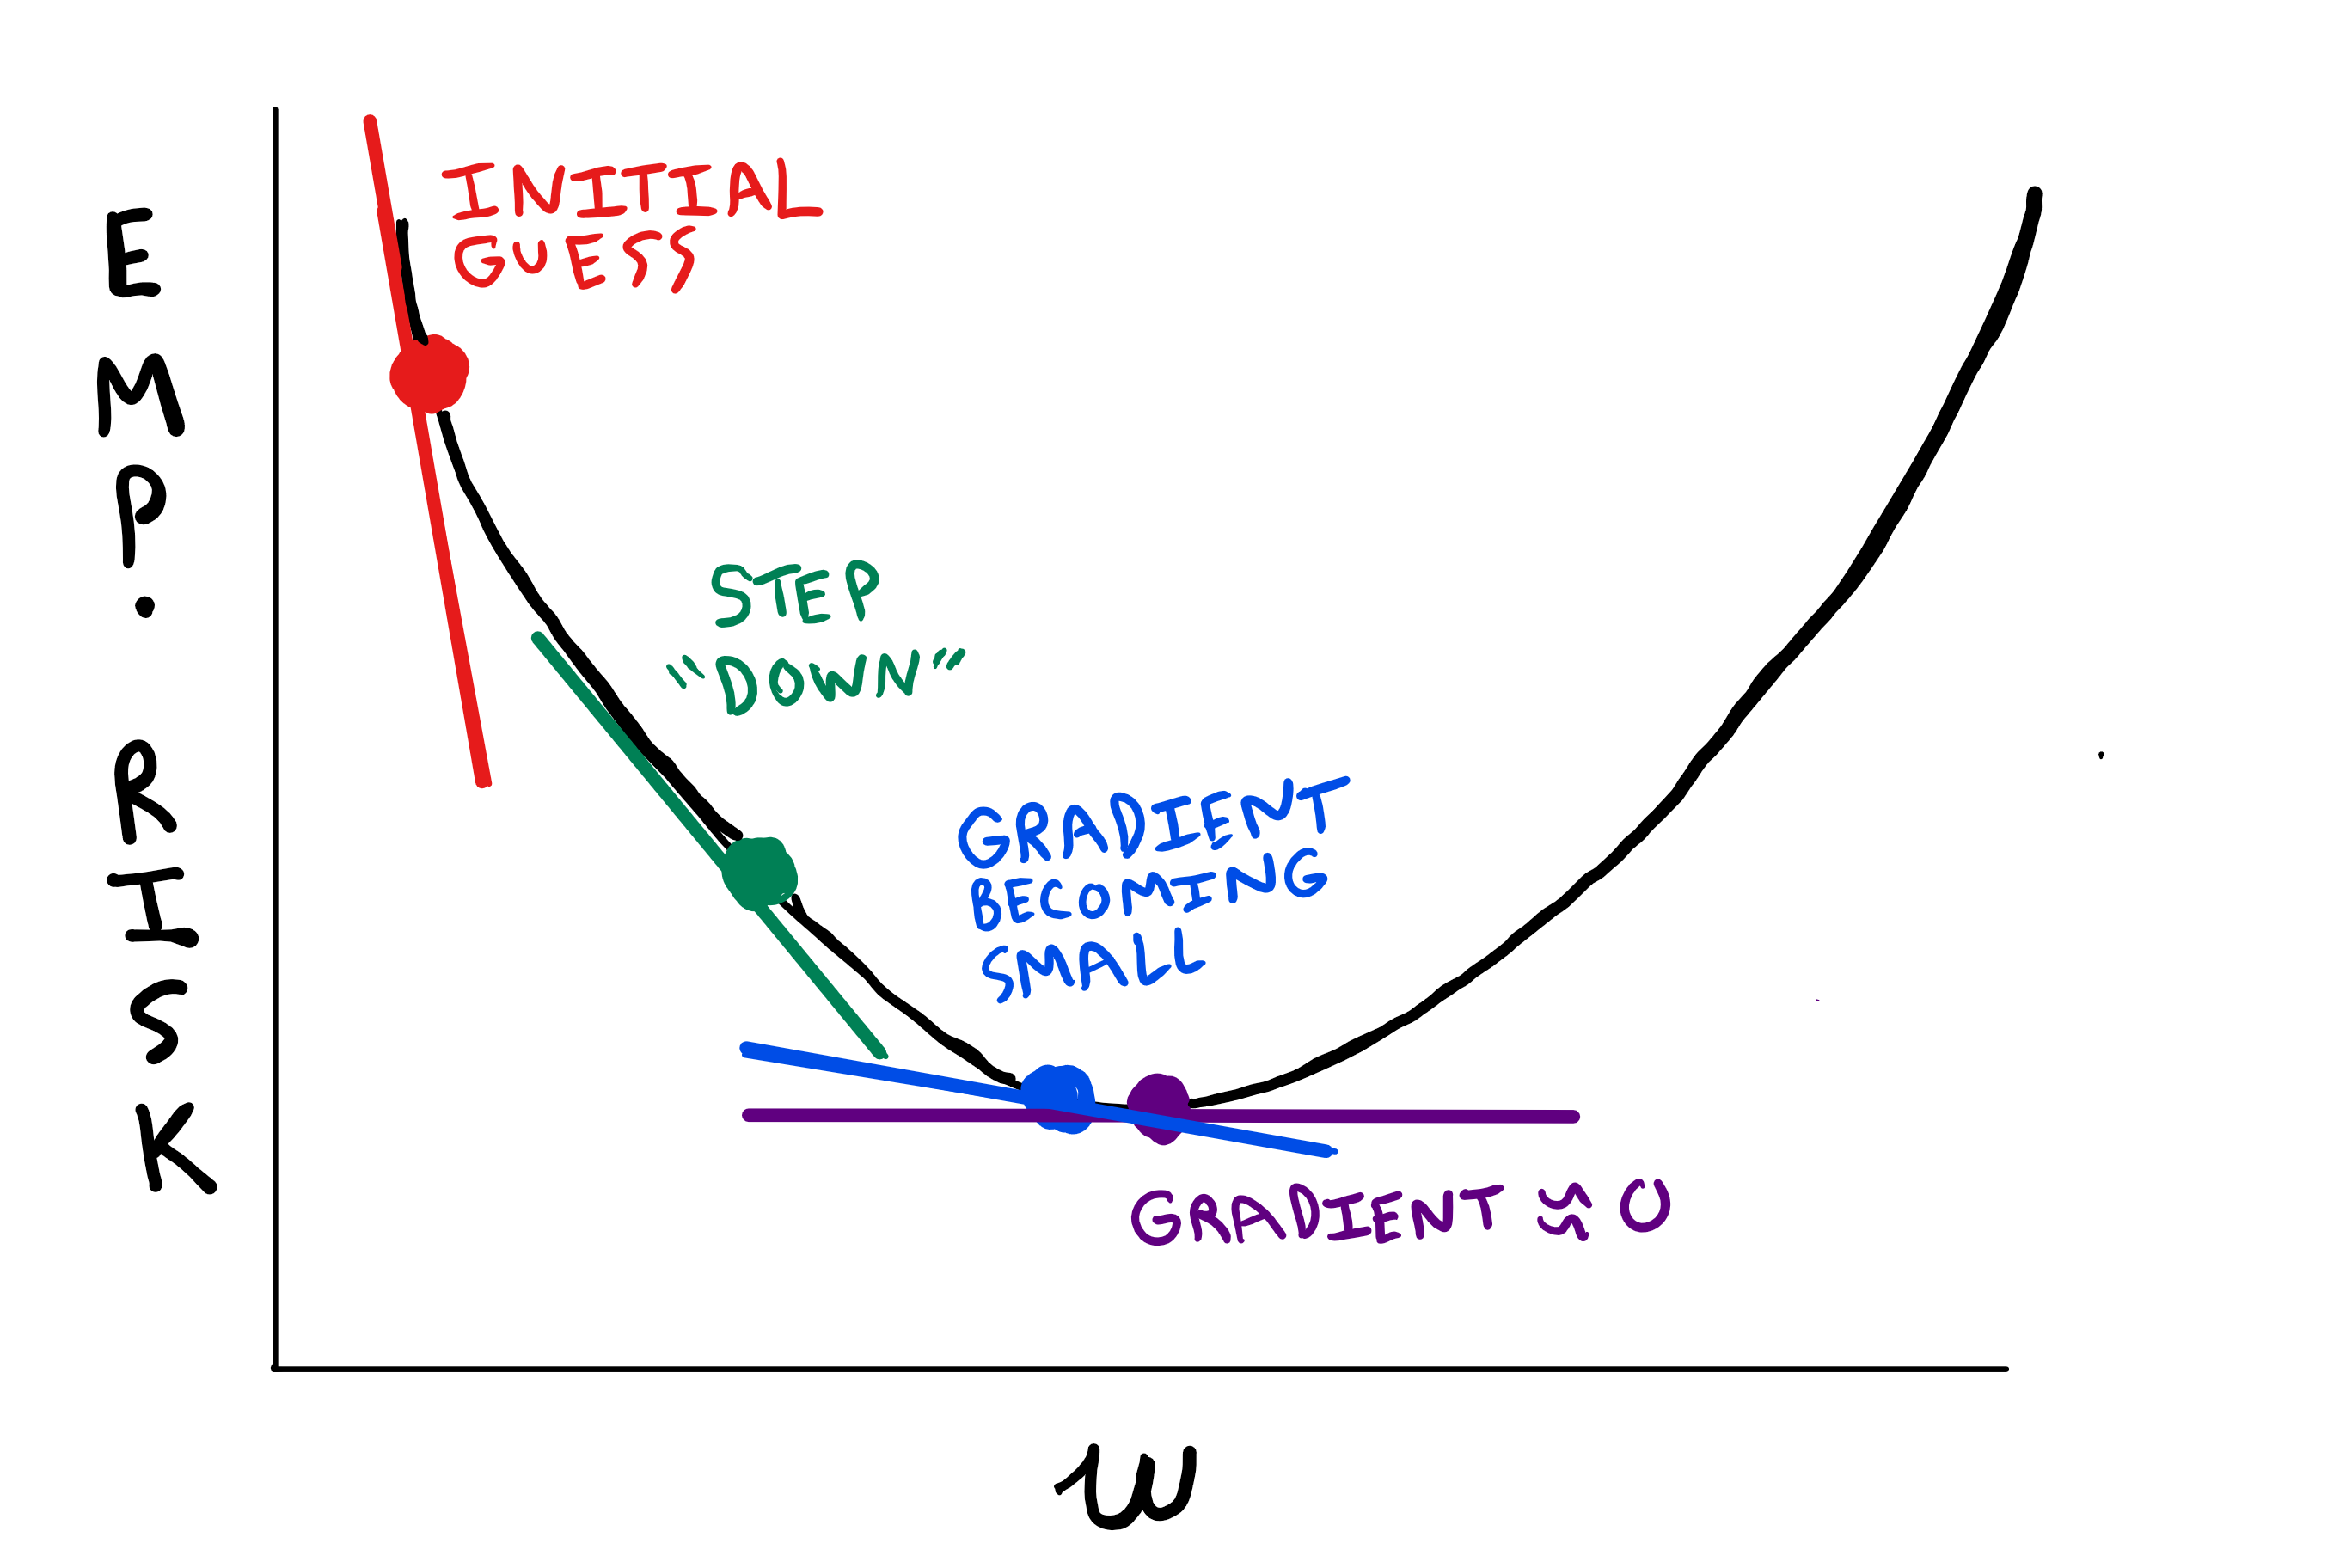
\includegraphics[scale=0.33]{Sketch}
	\end{figure}
\end{frame}

\begin{frame}
	\frametitle{A more formal explanation}

	$\mathbf{w}_{t+1} = \mathbf{w}_t - \gamma \frac{1}{n}\sum_{i=1}^n
	\nabla_w L(f_w(\mathbf{X}_i), y_i)$ \\~\\

	Stop if gradient $\leq \epsilon$ \\~\\

	Step size $\gamma$ can vary over time \\~\\

	Theoretical guarantees on speed of convergence ($\rho :=$ size of error):
	\begin{itemize}
		\item Version presented here: $ - \log \rho \sim t$
		\item More optimized version: $ - \log \log \rho \sim t$ \\~\\
	\end{itemize}
	
\end{frame}

\begin{frame}
	\frametitle{Batch gradient descent is computationally expensive}
	In ``plain'' (batch) gradient descent, for \textcolor{red}{every step}, 
	we have to evaluate the gradient at \textcolor{blue} {every observation}

	$$
	\textcolor{red}{\mathbf{w}_{t+1}} = \mathbf{w}_t - \gamma \frac{1}{n}
	\textcolor{blue}{\sum_{i=1}^n}
	\nabla_w L(f_w(\mathbf{X}_i), y_i)
	$$\\~\\

	This becomes computationally intractable as $n$ grows large 
	\begin{itemize}
		\item \small If we have $n$ = 10 million, we have to evaluate the
			gradient 10 million times for every step (and the
			algorithm may take many steps to converge)\\~\\
		\item \small May take hours or days to converge \\~\\
	\end{itemize}
\end{frame}

\begin{frame}
	\frametitle{Stochastic gradient descent (SGD) takes less time}

	For each step, gradient is computed for a \textcolor{red}{single} randomly
	chosen observation $i$:

	$$
	{\mathbf{w}_{t+1}} = \mathbf{w}_t - \gamma \nabla_w
	L(f_w(\mathbf{X}_{\textcolor{red}{i}}), y_{\textcolor{red}{i})}
	$$ \\~\\

	This simplification makes approximation much ``noisier'', and hence SGD
	requires more iterations \\~\\

	But, each iteration is faster and so SGD can reach a predefined
	level of risk or error in less time
\end{frame}

\begin{frame}
\frametitle{SGD is noisier than batch GD}
	\centering
	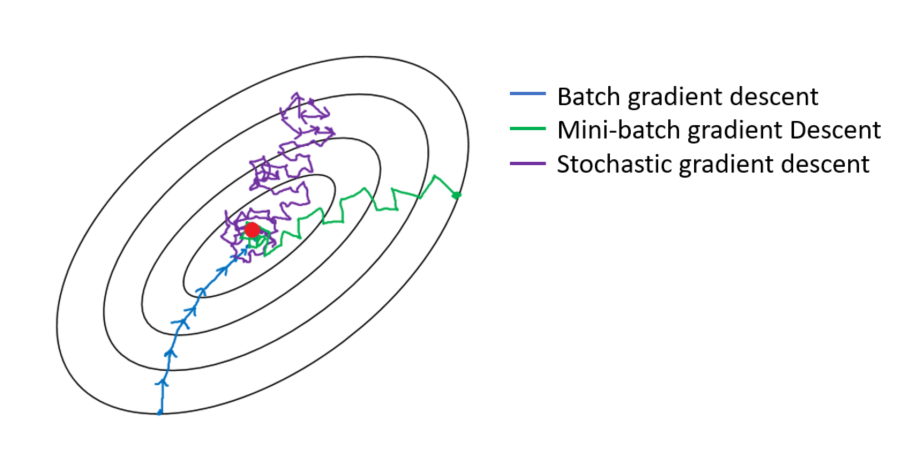
\includegraphics[scale=0.3]{noise}

	\tiny Source: towardsdatascience.com
\end{frame}

\begin{frame}
	\frametitle{SGD is useful when $n$ is large \& compute
	time is important}
	\begin{table}[t]
		\begin{tabular}{|l|c|c|}
			\hline
			& \textbf{GD} & \textbf{SGD} \\
			\textbf{Time to accuracy} $\mathbf{\rho}$ & $n \log
			\frac{1}{\rho}$ & $\frac{1}{\rho}$ \\
			\hline
		\end{tabular}
	\end{table}

	\begin{figure}
	\centering
	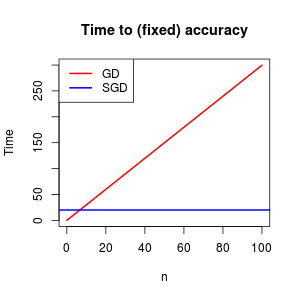
\includegraphics[scale=0.55]{comparison}
	\end{figure}

			
\end{frame}

\begin{frame}
	\frametitle{SGD is widely used in industry}
	If a Silicon Valley press release uses any of the following phrases...
	\begin{itemize}
		\item \small ``Neural networks''
		\item ``Machine learning''
		\item ``AI'' 
	\end{itemize}

	...SGD probably is involved. \\~\\
	
	Example: Google's \textbf{AlphaGo} program.
\end{frame}

\begin{frame}
	\begin{figure}[b]
	\centering
	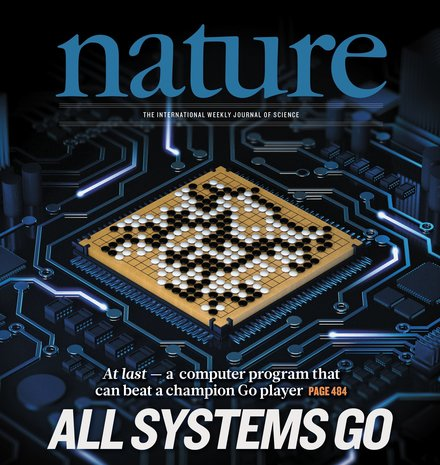
\includegraphics[scale=0.4]{go}
	\end{figure}
\end{frame}

\begin{frame}
	\frametitle{Google slides from ICML 2016}
	\centering
	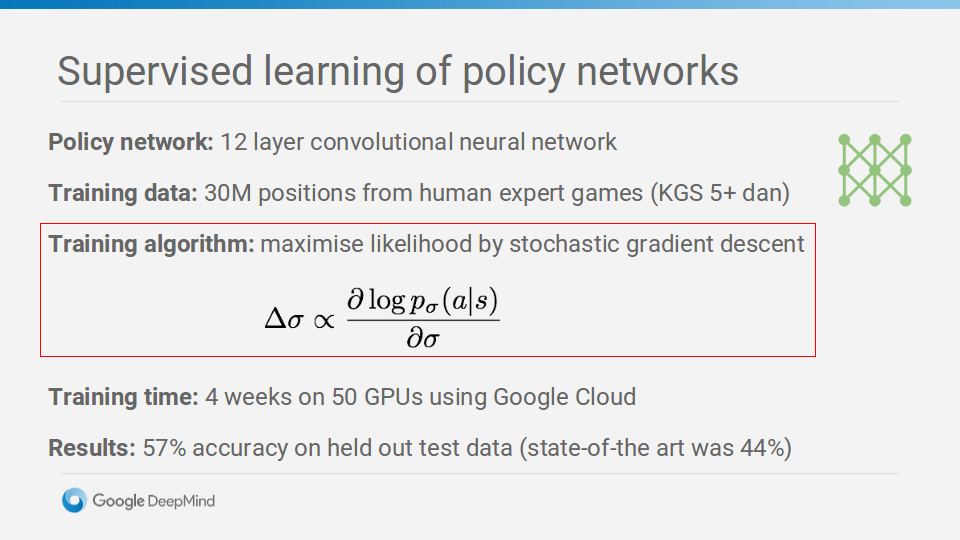
\includegraphics[scale=0.3]{screenshot}
\end{frame}

\end{document}


